\documentclass{atistandalonetask}
\usepackage{atistandard}

\begin{document}
  \begin{atiTask}[
    title = Sägezahnschwingung
  ]


	\begin{atiSubtasks}
		\item Berechnen Sie die Sinus-Cosinus-\textsc{Fourier}-Reihe der in der Abbildung gezeigten Sägezahnschwingung $f(t)$.
		\begin{figure}[H]
			\centering
			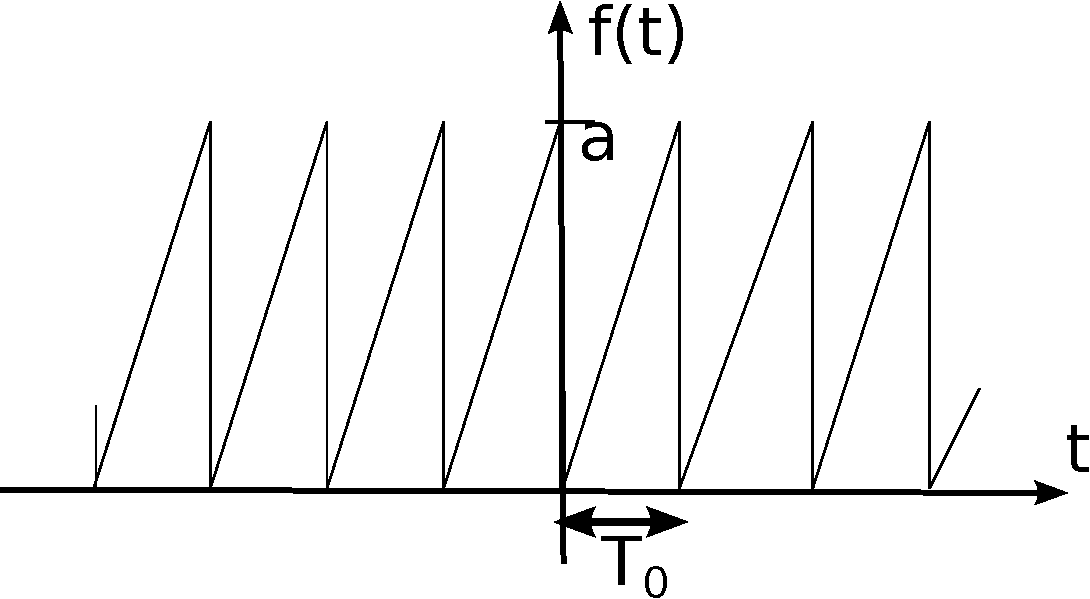
\includegraphics[width=0.70\linewidth]{picture-fourier_v}
			\caption{Sägezahnschwingung}
			\end{figure}
	%
		\item Bestimmen Sie die komplexe \textsc{Fourier}-Reihe dieser Funktion.
		\item \textbf{Zusatz für Interessierte und Punktesammler:} Die Funktion $f(t)$ sei die Erreger-Funktion eines gedämpften harmonischen Oszillators. Bestimmen Sie die \textsc{Fourier}-Reihe der Lösung $x(t)$ der Schwingungsgleichung
			\[
			m\leibnizDerivative[2]{x}{t}+\gamma \leibnizDerivative{x}{t}+kx=f.
			\]	
		Ist es einfacher, das Ergebnis von Aufgabenteil (a) oder das Resultat von Aufgabenteil (b) zu benutzen?	
	\end{atiSubtasks} 
  \end{atiTask}
  \begin{atiSolution}
      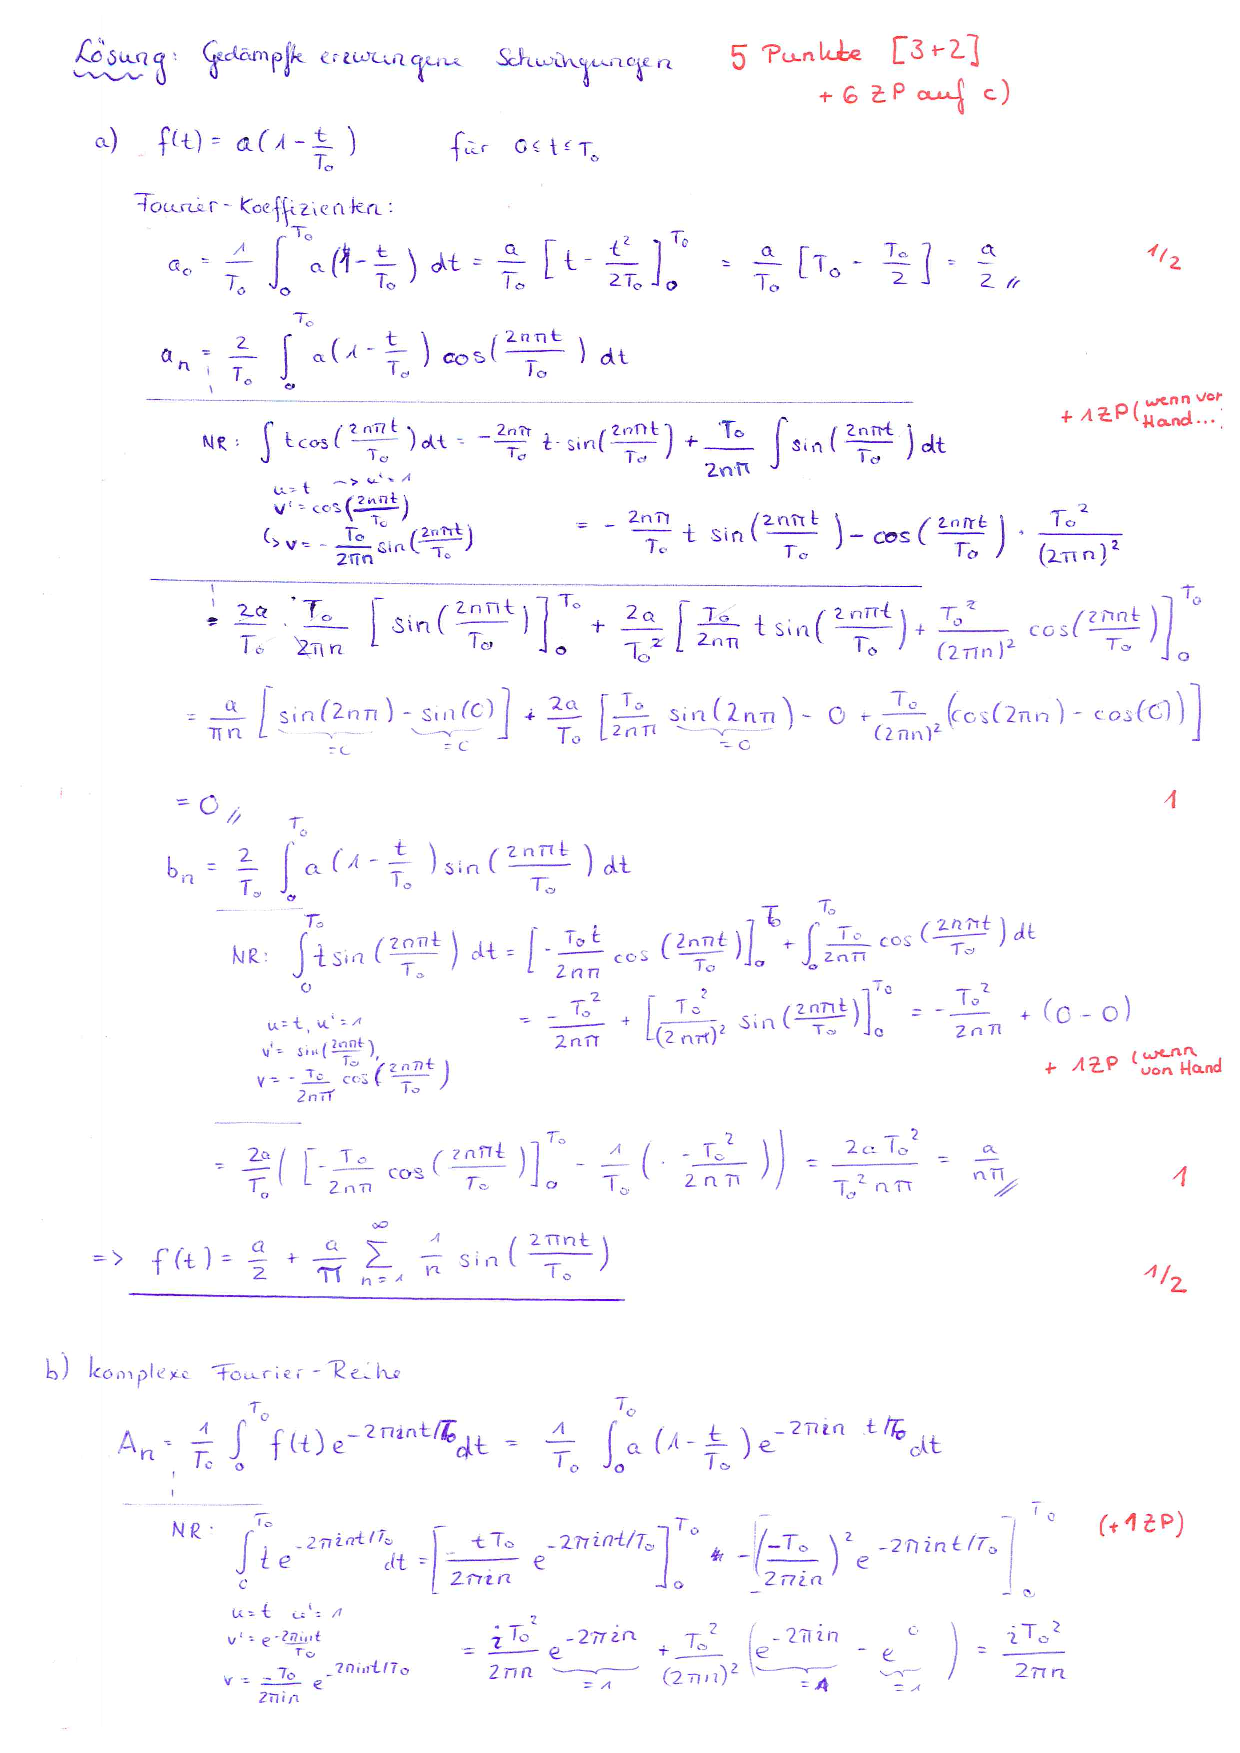
\includepdf[pages=-]{solution-fourier_v.pdf}
  \end{atiSolution}
\end{document}